\begin{figure*}[!h]
\begin{subfigure}{0.195\linewidth}
\centering
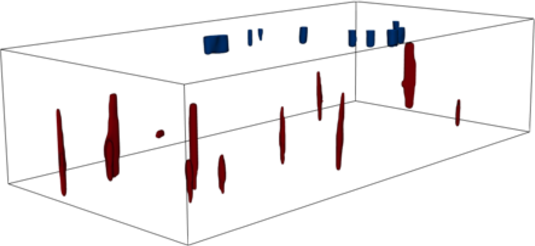
\includegraphics[width=\linewidth]{Images/Mantel/zls.pdf}
\vspace{-3mm}
\caption{$ZLS_{T}$}
\label{fig:mantel_zls}
\end{subfigure}
\begin{subfigure}{0.195\linewidth}
\centering
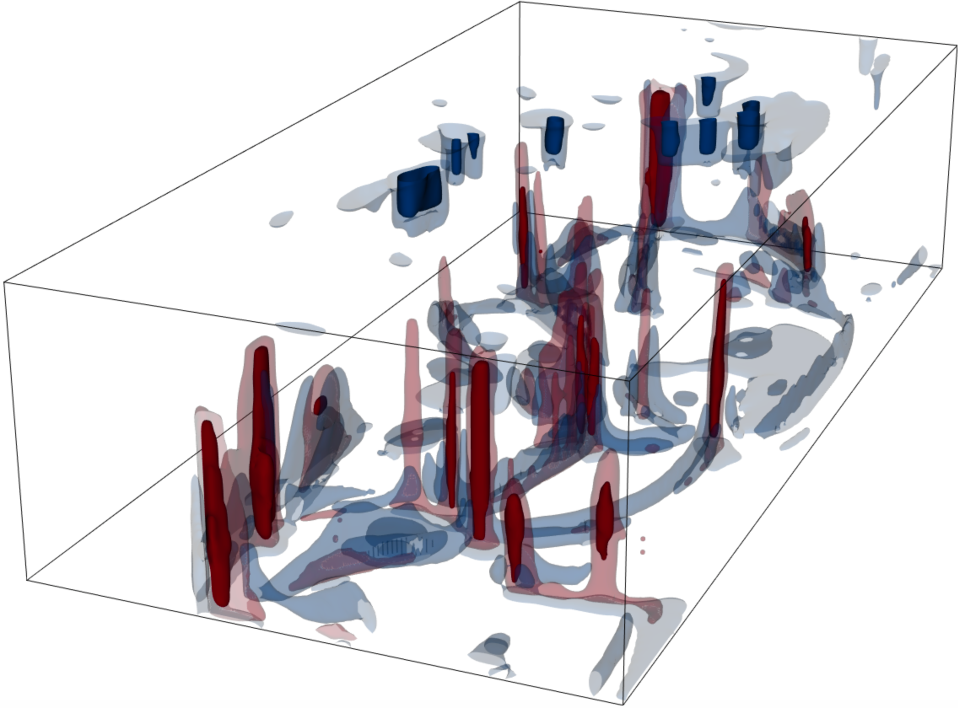
\includegraphics[width=\linewidth]{Images/Mantel/fcls_68.pdf}
\vspace{-3mm}
\caption{+ $FCLS_{T,68\%}$}
\label{fig:mantel_fcls_68}
\end{subfigure}
\begin{subfigure}{0.29\linewidth}
\centering
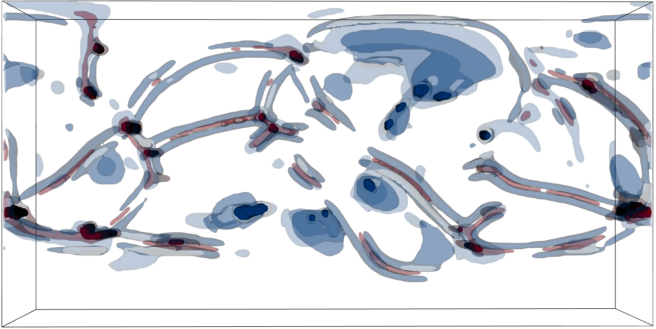
\includegraphics[width=0.9\linewidth]{Images/Mantel/fcls_68_v2.pdf}
\caption{View of $ZLS_{T}$ + $FCLS_{T,68\%}$ revealing the uncertain structure and spatial proximity of features identified by the selected traits.}
\label{fig:mantel_fcls_68_v2}
\end{subfigure}
\hfill
\begin{subfigure}{0.295\linewidth}
\centering
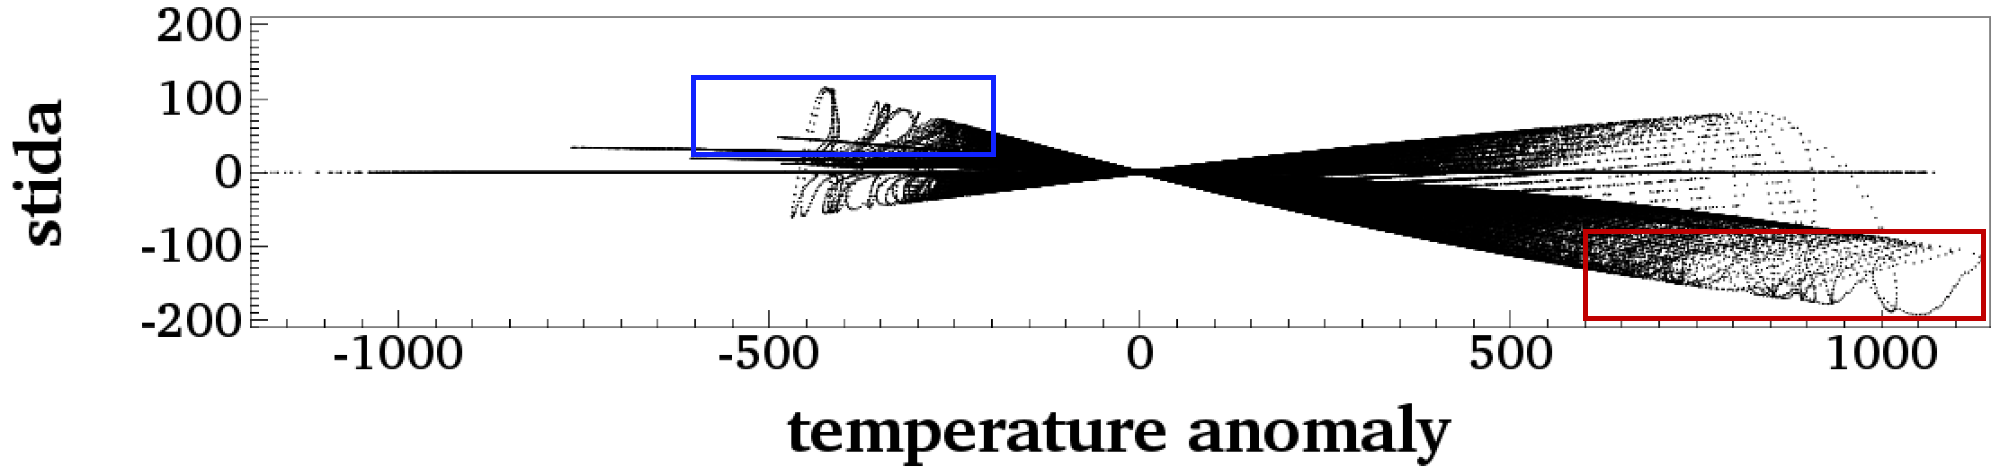
\includegraphics[width=\linewidth]{Images/Mantel/scatterplot.pdf}
%\vspace{-2mm}
\caption{2D scatterplot of $\mathcal{A}$ and traits. For the traits, we used extremes of temperature anomaly and negative spin-transition-induced density anomaly~(stida) to visualize flow patterns. We use $T = \left\{T_{A}, T_{B}\right\}$.} 
\label{fig:mantel_scatterplot}
\end{subfigure}
%\vspace{-2mm}
%\caption{Visualization of a subset of the spatial domain for the mantel data using temperature anomaly and spin-transition-induced density anomaly~(stida). We cosnidered extremes of temperature anomaly and negative spin-transition-induced density anomaly to visualize the flow patterns of rising hot plumes~($T_{A}$, red) and sinking material~($T_{B}$, blue) in the data.}
\caption{Visualization of rising hot plumes~($T_{A}$, red) and sinking material~($T_{B}$, blue) flow patterns in the Earth's mantel convection data using the temperature anomaly and spin-transition-induced density anomaly attributes. We considered a rectlinearly sampled mesh for a subset of the spatial domain.}
\label{fig:mantel}
\end{figure*}
